%----------------------------------------------------------------------------------------
%	Inställningar och dokumentkonfiguration
%----------------------------------------------------------------------------------------

\documentclass[paper=a4, fontsize=11pt]{report} % A4-sida och 11 punkters fontstorlek

\usepackage[T1]{fontenc} % 8-bitarskodning som har 256 glyfer
\usepackage[english]{babel} % Svenskt språk(ändrat till engelska)
\usepackage[utf8]{inputenc} % För svenska tecken
\usepackage{dtk-logos} % Logos
\usepackage{wallpaper} % Bakgrundsbild
\usepackage{fancyhdr} % Specialsidhuvud och sidfot
\usepackage{enumerate} 
\usepackage{hyperref}
\usepackage{textcomp}
\usepackage{xifthen}% provides \isempty test
\pagestyle{fancyplain} % Använd sidhuvud och sidfot på alla sidor
\fancyhead[L]{Laboration 3 -- 1DV720 --  \the\year -- Server Administration I} % Titel till vänster i sidhuvud
\fancyhead[C]{} % Tomt i mitten
\fancyhead[R]{} % Tomt till höger
\fancyfoot[L]{{\color{gray}\textcopyright \ \the\year \ Jacob Lindehoff}} % Tomt till vänster
\fancyfoot[C]{}  % Tomt i mitten
\fancyfoot[R]{\thepage} % Sidnumrering till höger i sidfoten
\renewcommand\thesection{\arabic{section}} % Section beter sig som i dokumentklassen article

\newcommand{\win}[1]{Microsoft Windows Server\ifthenelse{\isempty{#1}}{}{ #1}}
\newcommand{\gui}[0]{``Server with a GUI''}
\newcommand{\core}[0]{Windows Server Core}
%----------------------------------------------------------------------------------------
%	TITLE SECTION
%----------------------------------------------------------------------------------------
\newcommand\BackgroundPic{
    \put(-50,-50){
    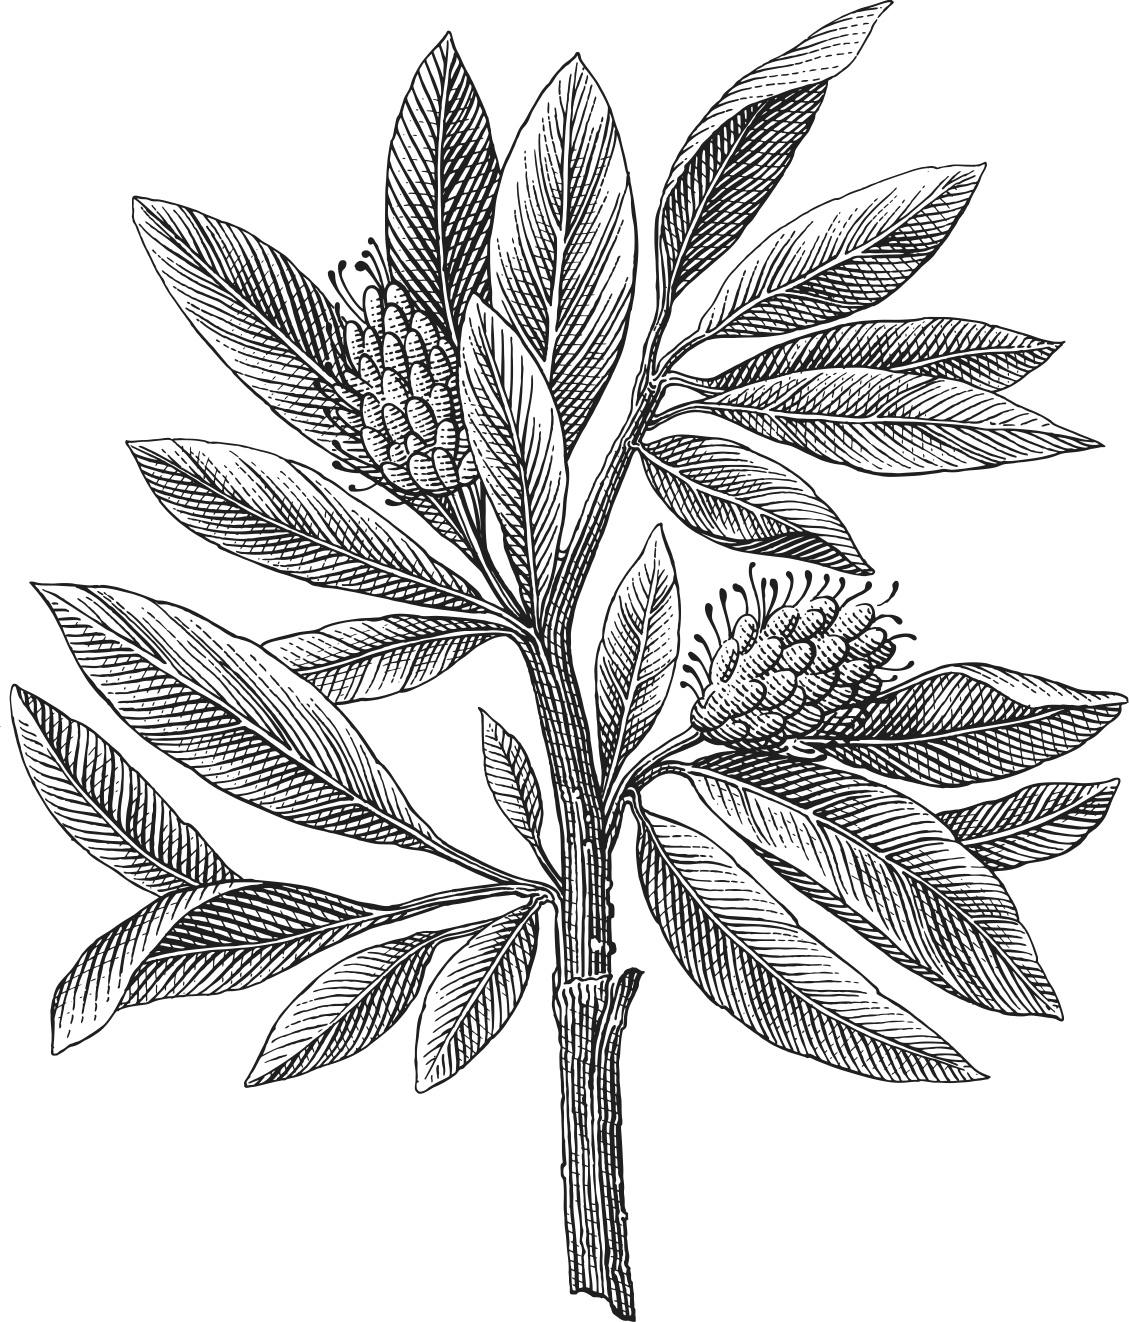
\includegraphics[keepaspectratio,scale=0.65]{lnu_etch.png} % Bakgrundsbild
    }
}
\newcommand\BackgroundPicLogo{
    \put(15,700){
    
\includegraphics[keepaspectratio,scale=0.10]{logo.png} % Logga i vänstra hörnet
    }
}

\newcommand{\horrule}[1]{\rule{\linewidth}{#1}} % Skapa hortisontell linje

\title{	\vspace{-10cm}
    \normalfont \normalsize
    \textsc{Linnaeus University} \\ [25pt] % Universitetes namn
    \horrule{0.5pt} \\[0.4cm] % Tunn linje högst upp
    \huge Laboration 3\\ % Arbetes titel
	\large \textcolor{gray}{1DV720 -- Server Administraion}
    \horrule{0.5pt} \\[0.4cm] % Tunn linje längst ner
}

% \author{Jacob Lindehoff} % Författarnas namn

\date{\normalsize\today} % Dagens datum

\begin{document}
\AddToShipoutPicture*{\BackgroundPic} % Lägger in backgrundsbild på första sidan
\AddToShipoutPicture*{\BackgroundPicLogo}
\maketitle % Skriv ut titeln
\noindent % Tabba inte in på första meningen

%------------------------------------------------
%	Introduction
%------------------------------------------------
\section{Introduction}

In this lab we will cover 2 very important services: DNS and a Web server - and see how they work together. As previously you will be using the lab environment from where you left off after lab 2. You will use the file server, in the DMZ that you created in lab 2, to store your web site files. 

Your will configure a web server that will serve a simple web site, the files will be stored on the file server. To be able to connect to the web site you should also configure DNS by setting up two name servers.

%------------------------------------------------
%	Deadline
%------------------------------------------------
\section{Deadline}

There are two laboratory sessions connected to this module, at these sessions you are given the opportunity to get help if so needed. To be able to finish the modules you are likely needed to spend more time on your own.

\paragraph{Accounting} You will show your work and demonstrate your progress at any of these lab session, prepare a small document with an overview of your configuration/setup if needed for overview.

\pagebreak
%------------------------------------------------
%	Uppgift
%------------------------------------------------
\section{Assignment}
\begin{figure}[h]
\centering
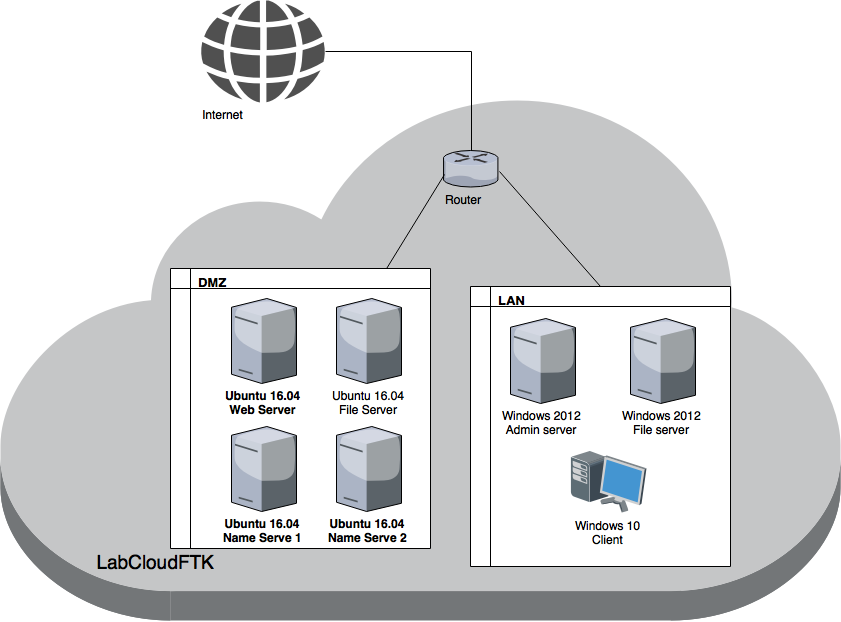
\includegraphics[width=1\linewidth]{./Lab03-Network}
\caption[Figure over network in Lab 3]{The network as it should be setup in Lab 3.}
\label{fig:network}
\end{figure}

In this lab you will only work in the DMZ network. The first thing you should focus on is setting up the name servers.
You'll need two name servers, one as master and the other as slave. You will configure them to answer for the domain \texttt{xx222yy.devopslab.xyz} where \texttt{xx222yy} is your LNU username.

When the zone is configured correctly you should register the domain name at \texttt{\href{https://www.devopslab.xyz}{https://www.devopslab.xyz}}. When that is done you should be able to  get answers for the domain from any where in the world.

Then you will setup a web server and configure a web site for 

\texttt{www.xx222yy.devopslab.xyz} where \texttt{xx222yy} is your LNU username. The web sites files should not be stored on the web server, instead they will be hosted on the DMZ file server.
\pagebreak

\section{Requirements}
\label{tasks}
As in the previous labs, security is important and all machines should have there firewalls enabled. Firewall rules will be checked to be ‘decent’. Remember that if (as it should be) your firewall is properly setup you will need to make exception for the protocols you are implementing.
As previously your configuration should survive a reboot.

\begin{itemize}
    \item All machines should:
    \begin{itemize}
		\item should have internet access
		\item within the same network be able to ping each other
    	\item have a proper naming convention.
    \end{itemize}
	\item Specific machine requirements:
    \begin{itemize}
        \item \textbf{Name server 1}
        \begin{itemize}
			\item OS: Ubuntu 16.04
			\item Name server: Bind 9
			\item Only answer for configured zones
			\item Should not be configured to redirect queries it can't answer for
			\item \textbf{Master} server for the zone \texttt{xx222yy.devopslab.xyz} where \texttt{xx222yy} is your LNU username
			\item A correctly configured SOA record
			\item Default TTL and Negative Cache TTL should \textbf{300} seconds
        \end{itemize}  
        \item \textbf{Name server 2}
        \begin{itemize}
			\item OS: Ubuntu 16.04
			\item Name server Bind 9
			\item Only answer for configured zones
			\item Should not be configured to redirect queries it can't answer for
			\item \textbf{Slave} server for the zone \texttt{xx222yy.devopslab.xyz} where \texttt{xx222yy} is your LNU username
        \end{itemize}   
        \item \textbf{Web server}
        \begin{itemize}
			\item OS: Ubuntu 16.04
			\item Web server: Apache 2
			\item The DMZ file server share should be mounted
			\item Should serve the site \texttt{www.xx222yy.devopslab.xyz} where \texttt{xx222yy} is your LNU username
			\item the HTML files for the site should be stored on the file server share
        \end{itemize}  

    \end{itemize}
\end{itemize}

\section{Work Environment}
\label{environment}

You will be using FTK Lab Cloud to be able to accomplish this lab. You will find your credentials and tutorial on how to get started on this page: \href{https://coursepress.lnu.se/kurs/serveradministration/lab-cloud/}{https://coursepress.lnu.se/kurs/serveradministration/lab-cloud/}

For this lab I have also created a video tutorial with some basics for this lab. You'll find it on the \texttt{\href{https://coursepress.lnu.se/kurs/serveradministration/moduler/module-3/laboration}{course homepage}}.

Good luck!
\end{document}
